\scanpage{131}
% archive foliation: 130
soit les \unsure{cartiers|quartiers} d'\uline{oranges} d'ordre $n\geq1$
\figure{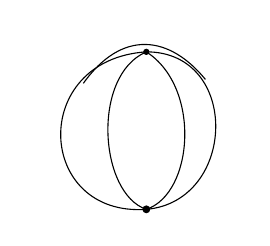
\begin{tikzpicture}[x=1cm,y=1cm]
\draw(0,1)..controls(-1.5,.9)and(-1.4,-1.1)..(0,-1);\draw(0,1)..controls(1.2,1)and(1.15,-.9)..(0,-1);\draw(0,1)..controls(-.7,.7)and(-.6,-.8)..(0,-1);\draw(0,1)..controls(.7,.55)and(.6,-.8)..(0,-1);\draw(-.8,.6)..controls(-.3,1.3)and(.3,1.2)..(.75,.65);\fill(0,1)circle(.04);\fill(0,-1)circle(.05);
\end{tikzpicture}}
-- mais si $n\geq2$, il n'y a pas
d'automorphismes hol. $\neq\operatorname{id}$.
Donc il semble que les seuls cas
où $\varphi$ ne soit pas unique sont les cas
(isomorphisme :) I) II), III) $=\mathrm{I}^*$) (\uline{NB} II) $=\mathrm{II}^*$)

Il faut cependant tirer au clair
entièrement l'argument de représentation
conforme, et voir s'il s'applique
aux cartes infinies.

Si on se donne en plus \deleted{les} l'ens
\deleted{pts de} $\varphi^{-1}(\{\infty\})$, \inserted{(centres des faces)}, alors les cas I) II) III)
sont éliminés. [Si on se donnait
$\varphi^{-1}(\{1\})$, celà éliminerait les cas
II et III, mais non le cas I\ldots]
